\chapter{Annexes}
\section{Configurer SQL Workbench/J pour se connecter à la base de données}
\label{sqlworkbenchj}

SQL Workbench/J est un client, écrit en Java (le même langage que celui utilisé pour écrire Alisma ou faire tourner la base de données en mode monoposte), qui permet d'interroger les bases de données SQL, quel qu'en soit leur type (MySQL, HSQLDB, PostgreSQL, etc.).

SQL est un langage normalisé qui permet d'interroger et de manipuler les bases de données. 

\underline{Attention} : bien que le nom soit quasi-identique, ce programme n'a rien à voir avec le logiciel SQL Workbench, fourni par MySQL.

\subsection{Installer et lancer SQL Workbench/J}

Téléchargez le logiciel depuis le site \url{http://www.sql-workbench.net/downloads.html}. Décompressez l'archive récupérée dans un dossier de votre poste de travail.

Lancez le logiciel en exécutant le programme \textit{SQLWorkbench64.exe}.

\subsection{Configurer le pilote permettant de dialoguer avec votre base de données}

Pour pouvoir gérer tout type de base de données, le logiciel a besoin de recourir à des pilotes adaptés. Cette configuration s'effectue depuis la fenêtre de connexion, en cliquant sur le bouton \textit{Manage Drivers}, en bas à gauche.

\subsubsection{Mode monoposte}
Recherchez dans la liste \textit{HSQLDB}. Dans la zone \textit{Library}, supprimez celle proposée, et remplacez-là par celle-ci : \textit{\NoAutoSpaceBeforeFDP c:\textbackslash{}alisma\textbackslash{}hsqldb\textbackslash{}lib\textbackslash{}hsqldb.jar}

\subsubsection{Mode réseau}

Recherchez dans la liste \textit{MySQL}. Dans la zone \textit{Library}, supprimez celle proposée, et remplacez-là par celle-ci : \textit{\NoAutoSpaceBeforeFDP c:\textbackslash{}alisma\textbackslash{}mysql\textbackslash{}mysql-connector-java-5.1.45-bin.jar}

\subsection{Configurer la connexion}

Pour vous connecter, indiquez les informations suivantes dans la fenêtre de connexion :
\subsubsection{Mode monoposte}
\begin{description}
\item [Driver] : HSQLDB
\item [URL] : {\NoAutoSpaceBeforeFDP jdbc:hsqldb:file:c:/alisma/data/alisma}
\item [Username] : SA
\item [Password] : vide
\end{description}

Vous pouvez enregistrer la configuration pour la conserver.

\subsubsection{Mode réseau}

\begin{description}
\item [Driver] : MySQL
\item [URL] : {\NoAutoSpaceBeforeFDP jdbc:mysql://localhost/alisma}
\item [Username] : alisma
\item [Password] : alisma
\end{description}

les informations de connexion peuvent varier en fonction de la configuration de la base de données. Consultez le cas échéant les paramètres indiqués dans le fichier \textit{param\textbackslash{}param.ini}.


%\section{Structure de la base de données}
%\includegraphics[width=\textwidth]{alismaPlaypen}
%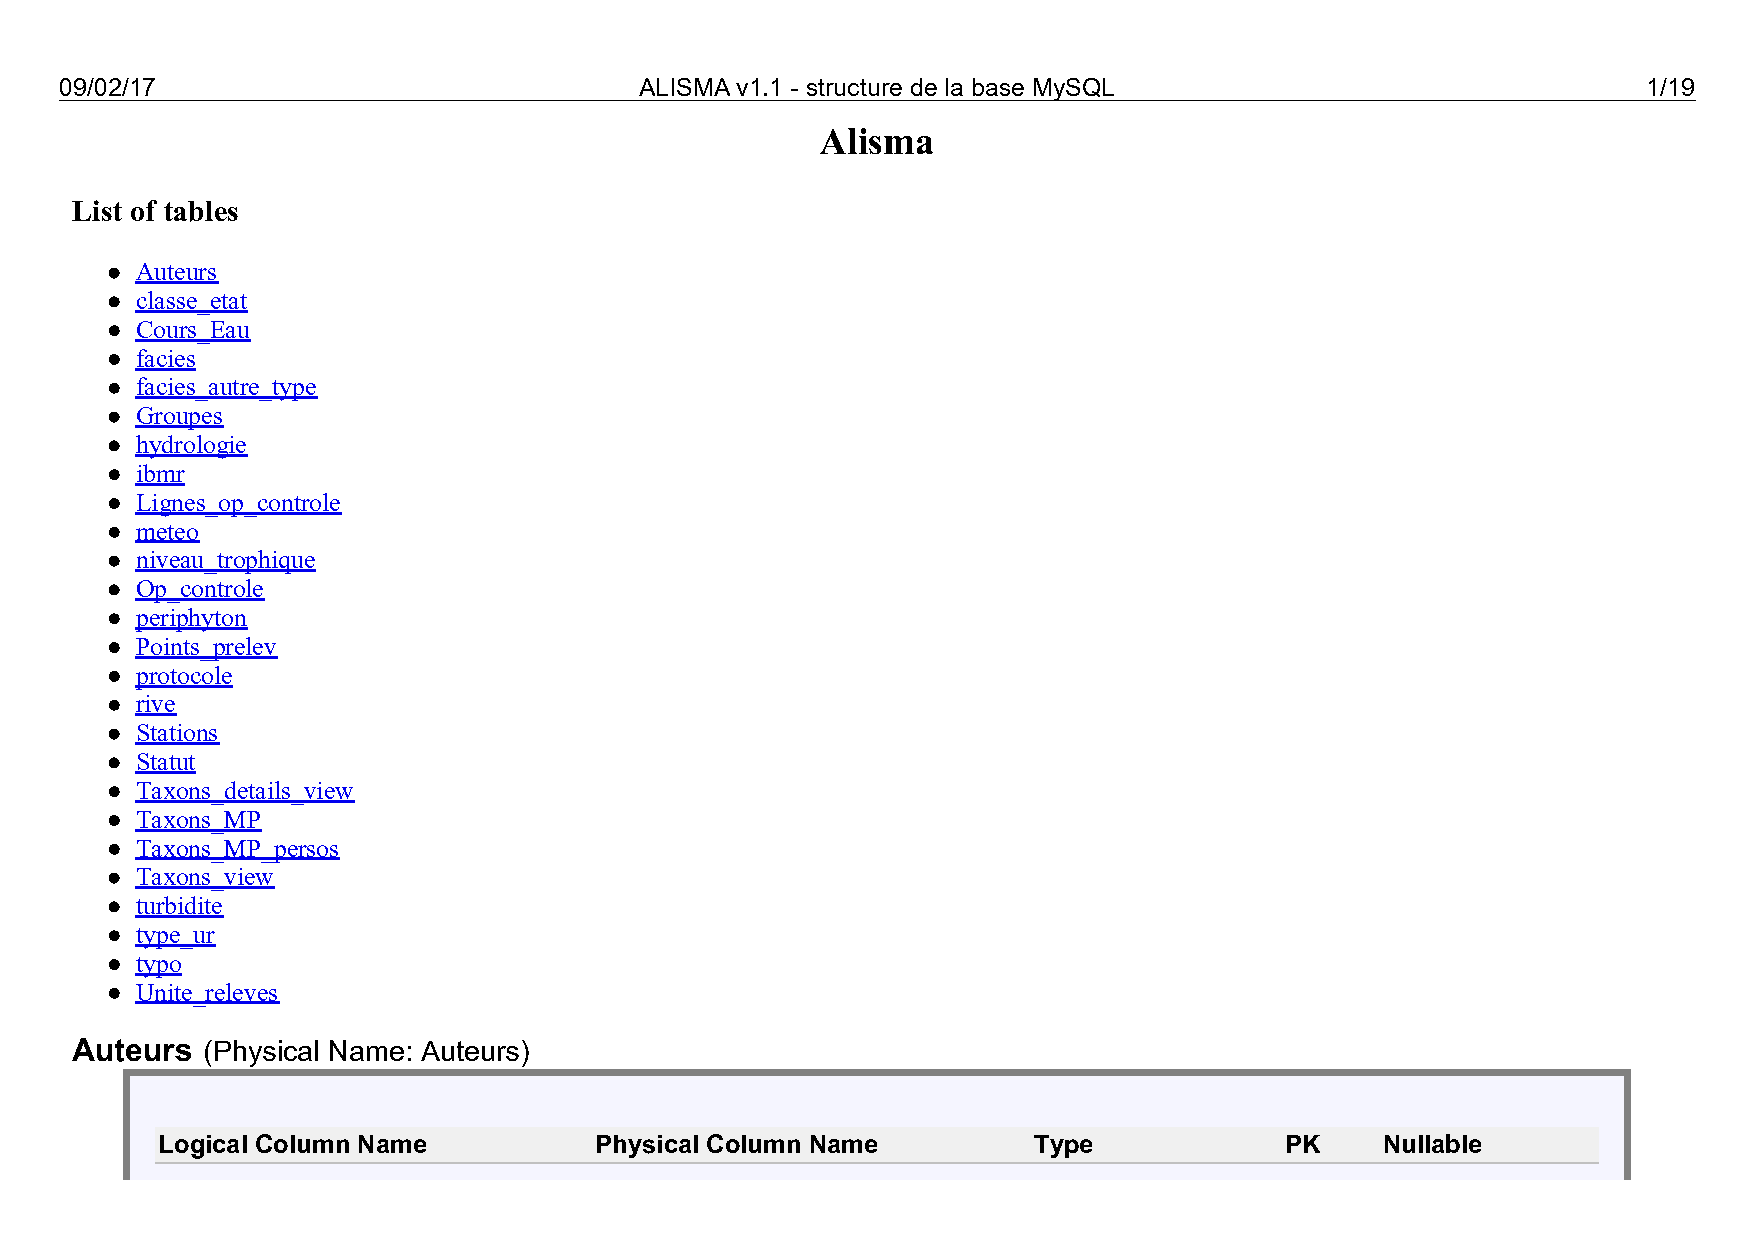
\includepdf[
%%pages=-,
%scale=.8,
%pagecommand={}
%]{alisma_structure.pdf}